\documentclass[a4paper]{article}
\usepackage[pdftex]{graphicx}
\usepackage{anysize}
\marginsize{3cm}{3cm}{3cm}{3cm}
\linespread{1.2}
\usepackage[utf8]{inputenc}
\usepackage[T1]{fontenc}       
\usepackage[swedish]{babel}      
\usepackage{epstopdf}     % För svensk avstavning och svenska
\usepackage[osf]{mathpazo} % Palatino with smallcaps and oldstyle numbers
\usepackage[scaled]{helvet}
\usepackage{morefloats} %så att man kan ha fler float-bilder
%\restylefloat{table}
\usepackage{etoolbox}
\usepackage{hanging}
\usepackage{listings}
\usepackage{graphicx}
\usepackage[width=.75\textwidth]{caption} %så all bildtext blir smalare

\lstset{language=SQL}

\newcommand\getcurrentref[1]{%
 \ifnumequal{\value{#1}}{0}
  {??}
  {\the\value{#1}}%
}  
\newcommand\requirement[2]{
	\numberedrow{Krav}{#1}{#2}
}
\newcommand\scenario[2] {
	\numberedrow{Scenario}{#1}{#2}
}
\newcommand\numberedrow[3]{
	\noindent
	\textbf{#1 \getcurrentref{section}.\getcurrentref{subsection}.#2.} #3
	
}

\usepackage{fancyhdr}
\fancyhf{}
\fancyhead[L]{Ansvarig: SG}

\fancyhead[R]{Datum: \today | Version: 0.2 | Dokumentnummer: PUSS144404}


\title{STLDD - Software Top Level Design Document: NewPussSystem}                  	
\author{Systemarkitektgruppen \\ Nina Khayyami | Johan Rönnåker |Martin Lichota | Marcel Tovar Rascon}
\date{}

\begin{document}

\maketitle
\thispagestyle{fancy}
\tableofcontents
\newpage

\section*{Dokumenthistorik}

\begin{tabular}{ l l l p{8.5cm} }
Ver. & Datum & Ansv. & Beskrivning \\\hline
0.1 & 30 september 2014 & SG & Struktur för dokumentet\\
0.2 & 2 oktober 2014 & SG & Lagt in klass-diagram, ER-diagram, sekvens-diagram samt lagt in all text. Färdigt för informell granskning.



\end{tabular}
\newpage
\section{Inledning}       
Dokumentet beskriver högnivådesignen för NewPussSystem, ett tidrapporteringssystem för projekt som diverse användare kan logga in på.



\section{Referensdokument}
\begin{enumerate}
\item SRS - Software Requirements Specification (Dokumentnummer PUSS144401, version 0.20)
\item STLDD - Software Top Level Design Document: BaseBlockSystem (Dokumentnummer PUSS12004, version 1.0)
\end{enumerate}



\section{Sammanfattning}
Systemet är implementerat i en Tomcat server med följande klasser och klassmetoder:

\subsection{Klasser}
\begin{hangparas}{1.5em}{1}
\textbf{class servletBase} Den här klassen är superklass åt alla servlets i systemet. För beskrivning se sidan 2 i dokumentet STLDD - Software Top Level Design Document: BaseBlockSystem.\end{hangparas} 

\vspace{5mm}
\begin{hangparas}{1.5em}{1}
\textbf{class Administration} Se sidan 2 i dokumentet STLDD - Software Top Level Design Document: BaseBlockSystem. En ändring har gjorts där metoden deleteUser ska returnera en boolean och inparametern ändras till (int id).\end{hangparas}

\vspace{5mm}
\begin{hangparas}{1.5em}{1}
\textbf{class ProjectGroupAdmin} Den här servleten ärver från ServletBase. Först kontrollerar den att användaren har behörighet att besöka sidan. Om så är fallet presenteras en tabell med information om varje projektgrupp (namn, projektledare, tidrapportmall). I tabellen kan administratören välja att radera gruppen och att lägga till/radera en projektledare. Projektgruppsnamnet i tabellen länkar administratören till projektledarens ändringsmeny. Nedanför tabellen finns en meny där administratören kan välja att lägga till nya projektgrupper (ny sida), gå tillbaka till startsidan för administration, gå tillbaka till den gemensamma första inloggningssidan, samt logga ut.\end{hangparas}

\vspace{5mm}
\begin{hangparas}{1.5em}{1}
\textbf{class TimeReporting} Den här servleten ärver från ServletBase och presenterar en submeny med specifika menyval relaterade till tidrapportering. Förutom submenyn kommer första sidan att vara tom. När ett val i submenyn görs, kommer klassen att hantera den valda funktionen. Funktionerna som finns inkluderar att lista tidrapporter, visa och uppdatera tidrapporter samt skapa nya tidrapporter.\end{hangparas}

\vspace{5mm}
\begin{hangparas}{1.5em}{1}
\textbf{class ReportGenerator} Den här statiska klassen har metoder som tar emot referenser till databasen och ritar upp en tidrapport med relevanta data. De olika tidrapporter som kan ritas upp är: en redigerbar, ny och tom tidrapport, en redigerbar existerande tidrapport och en icke redigerbar existerande tidrapport.\end{hangparas}

\vspace{5mm}
\begin{hangparas}{1.5em}{1}
\textbf{class ProjectLeader} Den här servleten ärver från ServletBase och visar automatiskt en lista över alla användare. Härifrån kan projektledaren antingen välja att hantera användaren i listan (lägga till, ta bort ur grupp) eller välja andra funktioner. \end{hangparas}

\vspace{5mm}
\begin{hangparas}{1.5em}{1}
\textbf{class ReportHandling} Den här servleten ärver från ServletBase och visar en lista med signerade och en lista med osignerade tidrapporter om man väljer att hantera tidrapporter. Projektledaren kan här signera eller avsignera rapporter.\end{hangparas}

\vspace{5mm}
\begin{hangparas}{1.5em}{1}
\textbf{class Statistics} Den här servleten ärver från ServletBase och visar vissa funktioner om man väljer att generera statistik. Funktioner som kan väljas är t.ex. att visa vilken vecka som det har tidrapporterats mest tid.\\ \end{hangparas}

\subsection{Klassmetoder}
Nedan beskrivs alla klassmetoder till klasserna som presenterats under rubriken 3.1 Klasser.

\subsubsection{class ProjectGroupAdmin}

\begin{hangparas}{1.5em}{1}
String addProjectForm()\\
Constructs a form for adding project groups.\\
@return String - The html-code for constructing the form.
\end{hangparas}

\vspace{5mm}
\begin{hangparas}{1.5em}{1}
private boolean addProject(String name, String leader, String timeReport)\\
Adds a new project group.\\
@param name: The name of the new project group.\\
@param leader: The name of the user that will be added as project 
leader to the project group.\\
@param timeReport: The time report template which will be used for 
the project group.\\
@return boolean: True if the group is added succesfully, else false.
\end{hangparas}

\vspace{5mm}
\begin{hangparas}{1.5em}{1}
private boolean deleteProject(int id)\\
Deletes a project group.\\
@param id: The id of the project group which will be deleted.\\
@return boolean: True if the group is deleted succesfully, else false.
\end{hangparas}

\vspace{5mm}
\begin{hangparas}{1.5em}{1}
private boolean addProjectLeader(String leaderName, String groupName)\\
Adds a project leader to a selected project group.\\
@param leaderName: The name of the user which will be added as project leader.\\
@param groupName: The project group to which the project leader will be added.\\
@return boolean: True if the project leader is added succesfully, else false.
\end{hangparas}

\vspace{5mm}
\begin{hangparas}{1.5em}{1}
private boolean removeProjectLeader(String leaderId, String groupId)\\
Removes a project leader from a selected project group.\\
@param leaderId: The id of the user which will be removed as project leader.\\
@param groupId: The id of the project group from which the project leader will be removed.\\
@return boolean: True if the project leader is removed succesfully, else false.\\
\end{hangparas}


\subsubsection{class TimeReporting}

\begin{hangparas}{1.5em}{1}
protected void printSubMenu()\\
Prints out a sub menu including the following option: view time reports and new time report.
\end{hangparas}

\vspace{5mm}
\begin{hangparas}{1.5em}{1}
protected void viewReportList()\\
Prints out a list of the user’s own reports.
\end{hangparas}

\vspace{5mm}
\begin{hangparas}{1.5em}{1}
protected void viewReport(String reportID)\\
Fetches the data for the time report specified by the String parameter and passes the data on to the static method viewReport in the static ReportGenerator class.\\
@param reportID: The id of the time report.
\end{hangparas}

\vspace{5mm}
\begin{hangparas}{1.5em}{1}
protected void printUpdateReport(String reportID)\\
Fetches the data for the time report specified by the String parameter and passes the data on to the static method updateReport in the static ReportGenerator class.\\
@param string: The id of the time report.
\end{hangparas}

\vspace{5mm}
\begin{hangparas}{1.5em}{1}
protected void printNewReport(int weekNumber)\\
Fetches the correct template from the database and passes it on to the static method newReport in the ReportGenerator class.\\
@param weekNumber: The weeknumber for the time report.
\end{hangparas}

\vspace{5mm}
\begin{hangparas}{1.5em}{1}
protected void updateReport(String reportID)\\
Updates the data stored in the database for the report specified by the String parameter.\\
@param string: The id of the time report to update.
\end{hangparas}

\vspace{5mm}
\begin{hangparas}{1.5em}{1}
protected void deleteReport(String reportID)\\
Deletes the report specified by the String parameter after confirmation and if and only if it is unsigned.\\
@param reportID: The id of the time report to delete.
\end{hangparas}

\vspace{5mm}
\begin{hangparas}{1.5em}{1}
protected void addNewReport()\\
Inserts the data from the new report form into the database.
\end{hangparas}

\vspace{5mm}
\begin{hangparas}{1.5em}{1}
protected void filterReportList(String filter)\\
Filters what time reposts that should be shown in the list.\\
@param filter: The filter that should be applied.\\
\end{hangparas}


\subsubsection{class ReportGenerator}

\begin{hangparas}{1.5em}{1}
public static void viewReport(ResultSet data)\\
Prints out a time report in the right format and with the data specified by the ResultSet parameter.\\
@param data: Specifies which data to print in the time report. 
\end{hangparas}

\vspace{5mm}
\begin{hangparas}{1.5em}{1}
public static void updateReport(ResultSet data)\\
Prints out a html-form in the right format and with the data specified by the ResultSet parameter.\\ 
@param data: Specifies which data to print in the html-form.
\end{hangparas}

\vspace{5mm}
\begin{hangparas}{1.5em}{1}
public static void newReport(int weekNumber)\\
Prints out a time report html-form prefilled with data.\\
@param weekNumber: Specifies for which week the data should be shown.\\
\end{hangparas}
 

\subsubsection{class ProjectLeader}

\begin{hangparas}{1.5em}{1}
public void showAllUsers()\\
Shows a list of all the users in the system.
\end{hangparas}

\vspace{5mm}
\begin{hangparas}{1.5em}{1}
public boolean assignRoleToUser(String user, String role)\\
Assigns a role to a user in a project group.\\
@param user: The user to be assigned a role.\\
@param role: Which role to assign.\\
@return boolean: True if the user was succesfully added, else false.
\end{hangparas}

\vspace{5mm}
\begin{hangparas}{1.5em}{1}
public boolean removeUserFromProject(String user)\\
Removes a user from a project group.\\
@param user: The user to be removed.\\
@return boolean: True if the user was successfully removed, else false.\\
\end{hangparas}


\subsubsection{class ReportHandling}

\begin{hangparas}{1.5em}{1}
private boolean signTimeReport( int timeReportID)\\
Signs a time report.\\
@param timeReportID: The id of the report that will be signed.\\
@return boolean: True if the time report was successfully signed, else false.
\end{hangparas}

\vspace{5mm}
\begin{hangparas}{1.5em}{1}
private boolean unsignTimeReport(int timeReportID)\\
Unsigns a time report.\\
@param timeReportID: The id of the report that will be unsigned.\\
@return boolean: True if the time report was succcessfully unsigned, else false.
\end{hangparas}

\vspace{5mm}
\begin{hangparas}{1.5em}{1}
private void showAllReports()\\
Shows a list of all the time reports.\\
\end{hangparas}


\subsubsection{class Statistics}

\begin{hangparas}{1.5em}{1}
private boolean generateStatisticsReport(String user, String role, String weeks, String activity)\\
Shows a time report based on the parameters requested by the user.\\
@param user: The user for the time report.\\
@param role: The role of the user(s) for the time report.\\
@param weeks: The weeks for which the time report will be shown.\\
@param activity: The activity that will be included in the time report.\\
@return boolean: True if the report was successfully generated and shown, else false.
\end{hangparas}

\vspace{5mm}
\begin{hangparas}{1.5em}{1}
private boolean generateSummarizedReport(List<String> timeReports, String activity, String subactivity)\\
Shows a time report with the summarized activity from several time reports.\\
@param timeReports: The time reports which it will summarize from.\\
@param activity: The activity which will be summarized.\\
@param subactivity: The subactivity which will be summarized.\\
@return boolean: True if the time report was successfully generated, else false.
\end{hangparas}

\vspace{5mm}
\begin{hangparas}{1.5em}{1}
private String commonActivity()\\
Finds the activity that has the most combined minutes reported by the users in the project group.\\
@return string: Returns the activity.
\end{hangparas}

\vspace{5mm}
\begin{hangparas}{1.5em}{1}
private int busiestWeek()\\
Finds the week with the most combined minutes reported by the users in the project group.\\
@return int: Returns the busiest week.\\
\end{hangparas}


\section{Klassdiagram}
Ett klassdiagram med alla klasser visas i Figur \ref{umldiagram}.

\begin{figure}[h!]
\centering
\includegraphics[width=90mm]{UML_hela_2okt.jpg}
\caption{Klassdiagram över alla klasser i systemet. \label{umldiagram}}
\end{figure}



\section{Databas}

ER-diagram över databasen för systemet visas i figur \ref{ER}. Databasen kan skapas från scratch med följande SQL kommandon: \\

\begin{figure}[ht!]
\centering
\includegraphics[width=120mm]{DB__1___9_.png}
\caption{ER-diagram över databasen för systemet \label{ER}}
\end{figure}

\begin{lstlisting}
mysql> create database base;
mysql> use base;
mysql> create table users (id int AUTO_INCREMENT, username varchar(10) UNIQUE, 
    -> password varchar(10), is_admin tinyint, is_project_leader tinyint, 
    -> is_logged_in tiny_int);
mysql> create table groups (id int AUTO_INCREMENT, name varchar(50) UNIQUE);
mysql> create table user_group (id int AUTO_INCREMENT, user_id int, group_id int,
    ->  role varchar(50), PRIMARY KEY (id), INDEX user_ind (user_id), 
    -> INDEX group_ind (group_id), FOREIGN KEY (user_id) REFERENCES users(id) ON 
    -> DELETE RESTRICT, FOREIGN KEY (group_id) REFERENCES groups(id) ON 
    -> DELETE RESTRICT);
mysql> create table log (id int AUTO_INCREMENT, user_id int, time timestamp, 
    -> session varchar(100), INDEX userlog_ind (user_id), FOREIGN KEY (user_id) 
    -> REFERENCES users(id) ON DELETE RESTRICT);
mysql> create table reports (id int AUTO_INCREMENT, user_group_id int,
    -> date date, week int, total_time int, signed tinyint, PRIMARY KEY (id),
    -> INDEX usergroup__ind (user_group_id), FOREIGN KEY (user_group_id) 
    -> REFERENCES user_group(id) ON DELETE RESTRICT);
mysql> create table times (id int AUTO_INCREMENT, report_id int,
    -> SDP_U int, SDP_I int, SDP_F int, SDP_O int, SRS_U int, SRS_I int,
    -> SRS_F int, SRS_O int, SVVS_U int, SVVS_I int, SVVS_F int, SVVS_O int,
    -> STLDD_U int, STLDD_I int, STLDD_F int, STLDD_O int, SVVI_U int,
    -> SVVI_I int, SVVI_F int, SVVI_O int, SDDD_U int, SDDD_I int, SDDD_F int,
    -> SDDD_O int, SVVR_U int, SVVR_I int, SVVR_F int, SVVR_O int, SSD_U int,
    -> SSD_I int, SSD_F int, SSD_O int, Slutrapport_U int, Slutrapport_I int,
    -> Slutrapport_F int, Slutrapport_O int, Funktionstest int, Systemtest int,
    -> Regressionstest int, Meeting int, Lecture int, Excersice int, Terminal int,
    -> Study int, Other int, PRIMARY KEY (id), INDEX timereport_ind (report_id),
    -> FOREIGN KEY (report_id) REFERENCES reports(id) ON DELETE RESTRICT);
mysql> insert into users (username, password, is_admin, is_project_leader, 
    -> is_logged_in) values('admin', 'adminpw', 1, 0, 0);


\end{lstlisting}


\section{Information lagrad i sessioner}
I en pågående session sparas följande attribut i sessionen:

\vspace{5mm}
\begin{hangparas}{1.5em}{1}
\textbf{Boolean tillstånd}: används för att beskriva om användaren är inloggad eller inte. Följande två tillstånd har definierats:\\
\textbf{true} inloggad\\
\textbf{false} utloggad
\end{hangparas}

\vspace{5mm}
\begin{hangparas}{1.5em}{1}
\textbf{Timestamp log} En tidsstämpel som indikerar när användaren senast gjorde en förfrågan i systemet.
\end{hangparas}

\vspace{5mm}
\begin{hangparas}{1.5em}{1}
\textbf{String name}: Användarens användarnamn, e.g. 'admin'. 
\end{hangparas}




\section{Sekvensdiagram}
\subsection{class Administration}
Figur 2 i dokumentet STLDD - Software Top Level Design Document: BaseBlockSystem visar sekvensen för hur servleten Administration hanterar att administratören lägger till en ny användare.


\subsection{class ProjectGroupAdmin}
Figur \ref{addGroup} visar hur servleten ProjectGroupAdmin hanterar en förfrågan om att lägga till en ny projektgrupp och Figur \ref{addGroupFail} visar hur den hanteras när den misslyckas.\\
Figur \ref{addProjectLeader} visar hur servleten ProjectGroupAdmin hanterar en förfrågan att lägga till en projektledare i ett projekt och Figur \ref{addProjectLeaderFail} visar hur det hanteras när den misslyckas, medans Figur \ref{removeProjectLeader} samt Figur \ref{removeProjectLeaderFail} visar hur servleten ProjectGroupAdmin hanterar en förfrågan att ta bort en projektledare då den lyckas samt då den misslyckas.\\
Figur \ref{removeGroup} visar hur servleten ProjectGroupAdmin hanterar en förfrågan om att ta bort en projektgrupp.

\begin{figure}[h!]
\centering
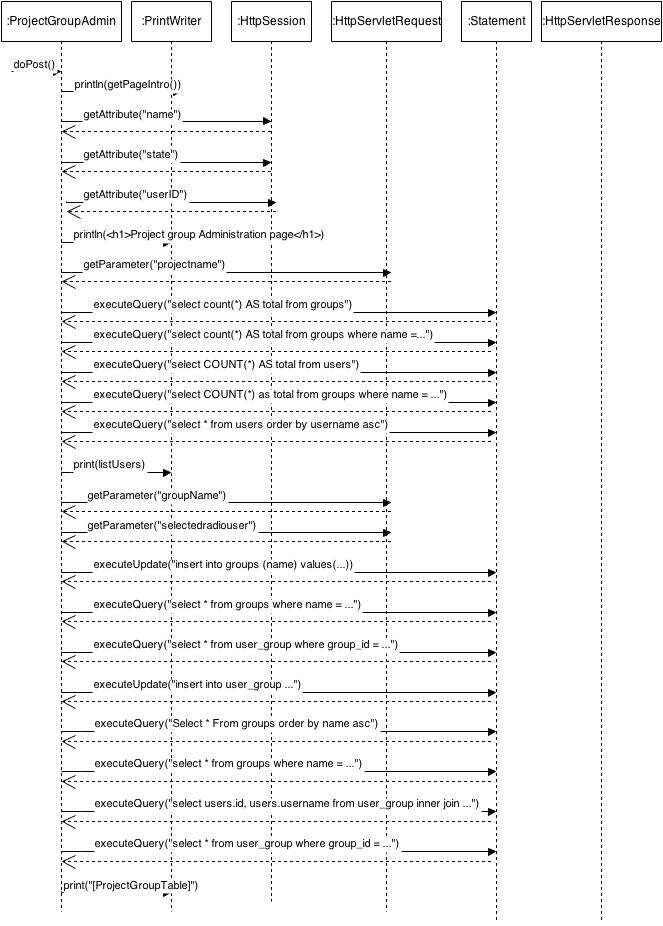
\includegraphics[width=90mm]{SeqDia__addGroup_FINAL.jpg}
\caption{Sekvensdiagram som visar hur en lyckad förfrågan om att lägga till en ny projektgrupp hanteras i klassen ProjectGroupAdmin. (Observera att inte alla meddelanden visas i sekvensen, utan endast dom som krävs för att förstå diagrammet.) \label{addGroup}}
\end{figure}

\begin{figure}[h!]
\centering
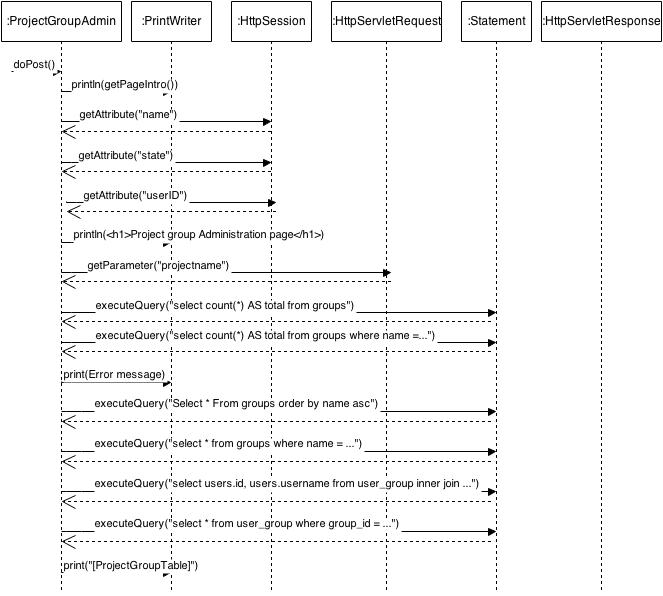
\includegraphics[width=90mm]{SeqDia__addGroup_Fail_FINAL.jpg}
\caption{Sekvensdiagram som visar hur en misslyckad förfrågan om att lägga till en ny projektgrupp hanteras i klassen ProjectGroupAdmin. (Observera att inte alla meddelanden visas i sekvensen, utan endast dom som krävs för att förstå diagrammet.) \label{addGroupFail}}
\end{figure}

\begin{figure}[h!]
\centering
\includegraphics[width=90mm]{SeqDia__addProjectLeader_FINAL.jpg}
\caption{Sekvensdiagram som visar hur klassen ProjectGroupAdmin hanterar en lyckad föfrågan om att lägga till en projektledare i en projektgrupp. (Observera att inte alla meddelanden visas i sekvensen, utan endast dom som krävs för att förstå diagrammet.) \label{addProjectLeader}}
\end{figure}

\begin{figure}[h!]
\centering
\includegraphics[width=90mm]{SeqDia__addProjectLeader_Fail_FINAL.jpg}
\caption{Sekvensdiagram som visar hur klassen ProjectGroupAdmin hanterar en misslyckad föfrågan om att lägga till en projektledare i en projektgrupp. (Observera att inte alla meddelanden visas i sekvensen, utan endast dom som krävs för att förstå diagrammet.) \label{addProjectLeaderFail}}
\end{figure}

\begin{figure}[h!]
\centering
\includegraphics[width=90mm]{SeqDia__removeProjectLeader_FINAL.jpg}
\caption{Sekvensdiagram som visar hur klassen ProjectGroupAdmin hanterar en lyckad föfrågan om att ta bort en projektledare i en projektgrupp. (Observera att inte alla meddelanden visas i sekvensen, utan endast dom som krävs för att förstå diagrammet.) \label{removeProjectLeader}}
\end{figure}

\begin{figure}[h!]
\centering
\includegraphics[width=90mm]{SeqDia__removeProjectLeader_fail_FINAL.jpg}
\caption{Sekvensdiagram som visar hur klassen ProjectGroupAdmin hanterar en misslyckad föfrågan om att ta bort en projektledare i en projektgrupp. (Observera att inte alla meddelanden visas i sekvensen, utan endast dom som krävs för att förstå diagrammet.) \label{removeProjectLeaderFail}}
\end{figure}

\begin{figure}[h!]
\centering
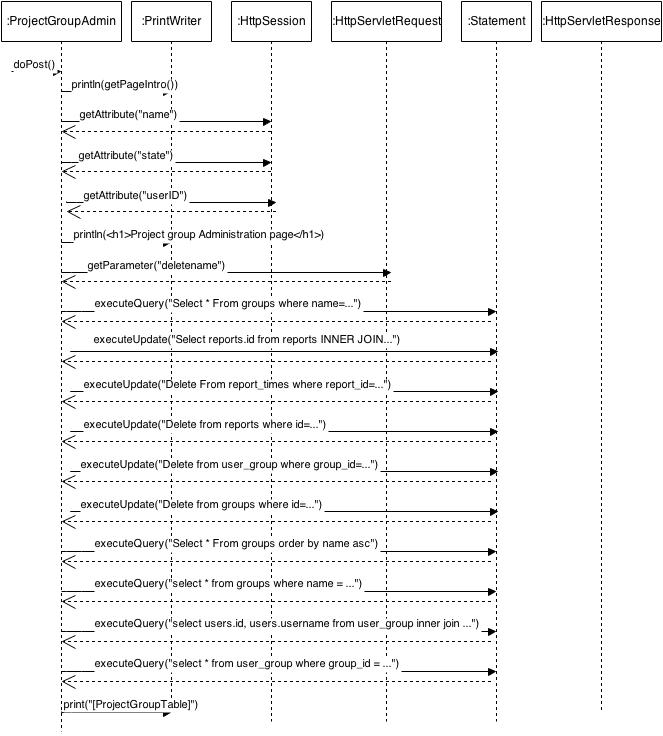
\includegraphics[width=90mm]{SeqDia__removeGroup_FINAL.jpg}
\caption{Sekvensdiagram som visar hur klassen ProjectGroupAdmin hanterar en förfrågan om att ta bort en projektgrupp. (Observera att inte alla meddelanden visas i sekvensen, utan endast dom som krävs för att förstå diagrammet.)\label{removeGroup}}
\end{figure}


\subsection{TimeReporting}
Figur \ref{newReport} visar hur servleten TimeReporting hanterar en förfrågan om att skapa en ny tidrapport som läggs till i databasen.\\
Figur \ref{removeReport} visar hur servleten TimeReporting hanterar en förfrågan om att ta bort en tidrapport och Figur \ref{removeReportFail} visar hur det hanteras när den misslyckas.\\
Figur \ref{updateReportSigned} visar hur servleten TimeReporting hanterar en förfrågan om att uppdatera en tidrapport som redan blivit signerad och Figur \ref{updateReportUnsigned} visar hur en förfrågan om att uppdatera en tidrapport som ännu inte blivit signerad hanteras.\\
Figur \ref{viewReportList} visar hur servleten TimeReporting hanterar en förfrågan om att skriva ut en användares alla tidrapporter, Figur \ref{viewReportListFail} visar hur den hanteras när den misslyckas.

\begin{figure}[h!]
\centering
\includegraphics[width=90mm]{newReport_successful.jpg}
\caption{Visar sekvensen av de grundläggande metodanrop som sker då användaren framgångsrikt skapar en ny tidrapport i klassen TimeReporting. (Observera att inte alla meddelanden visas i sekvensen, utan endast dom som krävs för att förstå diagrammet.) \label{newReport}}
\end{figure}

\begin{figure}[h!]
\centering
\includegraphics[width=90mm]{removeReport_successful.jpg}
\caption{Visar sekvensen av de grundläggande metodanrop som sker i klassen TimeReporting då användaren framgångsrikt tar bort en tidrapport som inte är signerad. (Observera att inte alla meddelanden visas i sekvensen, utan endast dom som krävs för att förstå diagrammet.) \label{removeReport}}
\end{figure}

\begin{figure}[h!]
\centering
\includegraphics[width=90mm]{removeReport_unsuccessful.jpg}
\caption{Visar sekvensen av de grundläggande metodanrop som sker i klassen TimeReporting då användaren misslyckat försöker ta bort en tidrapport som är signerad. (Observera att inte alla meddelanden visas i sekvensen, utan endast dom som krävs för att förstå diagrammet.)\label{removeReportFail}}
\end{figure}

\begin{figure}[h!]
\centering
\includegraphics[width=90mm]{updateReport_signed.jpg}
\caption{Visar sekvensen av de grundläggande metodanrop som sker i klassen TimeReporting då användaren misslyckat försöker uppdatera en tidrapport som är signerad. (Observera att inte alla meddelanden visas i sekvensen, utan endast dom som krävs för att förstå diagrammet.)\label{updateReportSigned}}
\end{figure}

\begin{figure}[h!]
\centering
\includegraphics[width=90mm]{updateReport_unsigned.jpg}
\caption{Visar sekvensen av de grundläggande metodanrop som sker i klassen TimeReporting då användaren framgångsrikt uppdaterar en tidrapport som inte är signerad. (Observera att inte alla meddelanden visas i sekvensen, utan endast dom som krävs för att förstå diagrammet.)\label{updateReportUnsigned}}
\end{figure}

\begin{figure}[h!]
\centering
\includegraphics[width=90mm]{viewReportList_successful.jpg}
\caption{Visar sekvensen av de grundläggande metodanrop som sker i klassen TimeReporting då användaren framgångsrikt listar alla sina befintliga tidrapporter. (Observera att inte alla meddelanden visas i sekvensen, utan endast dom som krävs för att förstå diagrammet.) \label{viewReportList}}
\end{figure}

\begin{figure}[h!]
\centering
\includegraphics[width=90mm]{viewReportList_unsuccessful.jpg}
\caption{Visar sekvensen av de grundläggande metodanrop som sker i klassen TimeReporting då användaren misslyckat försöker lista alla sina befintliga tidrapporter, då denne inte har några befintliga tidrapporter. (Observera att inte alla meddelanden visas i sekvensen, utan endast dom som krävs för att förstå diagrammet.) \label{viewReportListFail}}
\end{figure}


\subsection{ProjectLeader}
Figur \ref{assignRole} visar hur servleten ProjectLeader hanterar en förfrågan om att tilldela en projektroll till en användare. Figur \ref{removeUserFromProject} visar hur servleten ProjectLeader hanterar en förfrågan om att ta bort en användare från en projektgrupp. 

\begin{figure}[h!]
\centering
\includegraphics[width=90mm]{assignRole.jpg}
\caption{Sekvensdiagram som beskriver hur klassen ProjectLeader hanterar en förfrågan om att tilldela en användare en projektroll. (Observera att inte alla meddelanden visas i sekvensen, utan endast dom som krävs för att förstå diagrammet.) \label{assignRole}}
\end{figure}

\begin{figure}[h!]
\centering
\includegraphics[width=90mm]{removeUserFromProject.jpg}
\caption{Sekvensdiagram som visar hur en förfrågan om att ta bort en användare från en projektgrupp hanteras i klassen ProjectLeader.(Observera att inte alla meddelanden visas i sekvensen, utan endast dom som krävs för att förstå diagrammet.) \label{removeUserFromProject}}
\end{figure}

\subsection{ReportHandling}

Figur \ref{showAllViewReport} visar hur servleten ReportHandling hanterar en förfrågan om att visa alla tidrapporter i projektgruppen, signerade samt osignerade. Figur \ref{signedReport} visar hur servleten ProjectLeader hanterar en förfrågan om att signera en rapport.

\begin{figure}[h!]
\centering
\includegraphics[width=90mm]{showAllViewReport.jpg}
\caption{Sekvensdiagram som visar hur klassen ReportHandling hanterar en förfrågan om att visa alla tidrapporter i en projektgrupp. (Observera att inte alla meddelanden visas i sekvensen, utan endast dom som krävs för att förstå diagrammet.) \label{showAllViewReport}}
\end{figure}

\begin{figure}[h!]
\centering
\includegraphics[width=90mm]{signedReport.jpg}
\caption{Sekvensdiagram som visar hur klassen ReportHandling hanterar en förfrågan om att signera en rapport. (Observera att inte alla meddelanden visas i sekvensen, utan endast dom som krävs för att förstå diagrammet.) \label{signedReport}}
\end{figure}

\subsection{Statistics}
Figur \ref{busiestWeek} visar hur servleten Statistics hanterar en förfrågan om att visa vilken vecka som har flest totala inlagda minuter.\\
Figur \ref{commonActivity} visar hur servleten Statistics hanterar en förfrågan om att visa vilken aktivitet som har flest totala inlagda minuter.\\
Figur \ref{generateStatisticsReport} visar hur servleten Statistics hanterar en förfrågan om att visa en tidrapport som sammanfattar arbetet utfört i en viss aktivitet av en viss grupp/undergrupp under en specifik tid.

\begin{figure}[h!]
\centering
\includegraphics[width=90mm]{busiestWeek.jpg}
\caption{Sekvensdiagram som visar hur en förfrågan om att visa vilken vecka som har flest totala inlagda minuter hanteras i klassen Statistics. (Observera att inte alla meddelanden visas i sekvensen, utan endast dom som krävs för att förstå diagrammet.) \label{busiestWeek}}
\end{figure}

\begin{figure}[h!]
\centering
\includegraphics[width=90mm]{commonActivity.jpg}
\caption{Sekvensdiagram som beskriver hur en förfrågan om att visa vilken aktivitet som har flest totala inlagda minuter hanteras i klassen Statistics. (Observera att inte alla meddelanden visas i sekvensen, utan endast dom som krävs för att förstå diagrammet.)\label{commonActivity}}
\end{figure}

\begin{figure}[h!]
\centering
\includegraphics[width=90mm]{generateStatisticsReport.jpg}
\caption{Sekvensdiagram som visar hur klassen Statistics hanterar en förfrågan om att visa en tidrapport som sammanfattar arbetet utfört i en viss aktivitet av en viss grupp/undergrupp under en specifik tid. (Observera att inte alla meddelanden visas i sekvensen, utan endast dom som krävs för att förstå diagrammet.) \label{generateStatisticsReport}}
\end{figure}

\end{document}